\section{Methods}
\label{sec:methods}

\subsection{Implementation}
\label{sec:methods:implementation}

\subsubsection{Design description and structural generation}
\label{sec:forge:architecture}
\label{sec:forge:contract-model}

The module registry lists the modules and their build recipes. Each module's interface contract maps physical ports to roles, and the topology names the instances and connects them. \forge{} validates these inputs and resolves them into an IR with a versioned schema (Figure~\ref{fig:forge:architecture}). The generators and latency checker read this IR. To verify an existing top, \forge{} can work directly from its RTL sources and reference data.

\begin{figure}[!htb]
  \centering
  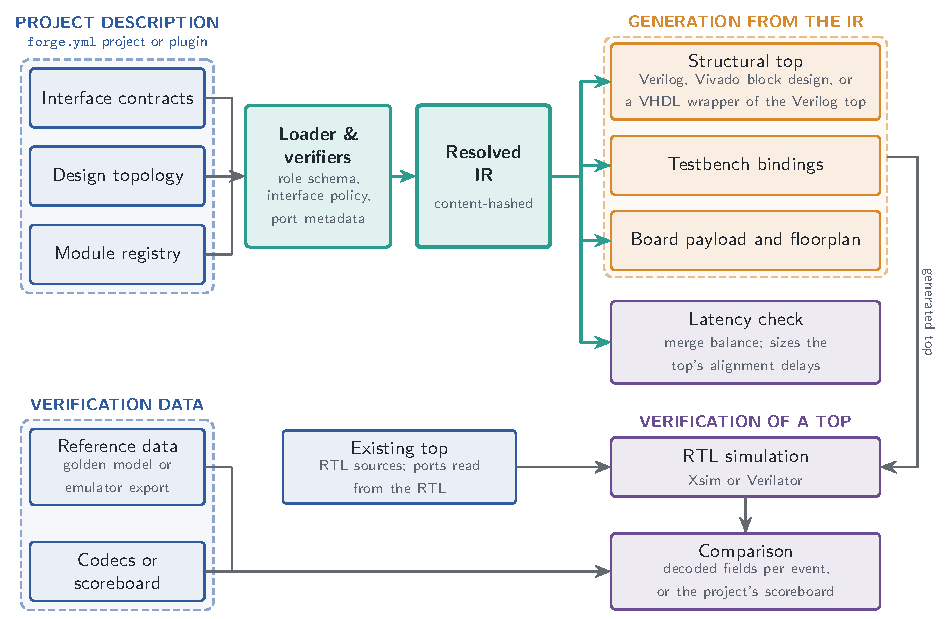
\includegraphics{figures/fig_forge_architecture}
  \caption{Design generation and RTL verification. Above, \forge{} resolves the design, generates the structural top, testbench bindings, and board payload, and sizes the alignment delays. Below, the simulator runs a generated or existing top. The verification flow compares its outputs with reference data using project codecs or a scoreboard.}
  \label{fig:forge:architecture}
\end{figure}

This excerpt from the \texttt{hit\_collector} contract in \texttt{trigger\_demo} shows the reset and four-element input array.

\begin{codeblock}
module_name: hit_collector
roles:
  reset_primary:
    raw_port: ap_rst
    direction: input
    width: 1
    active_level: high
  input_hit_array:
    array: true
    raw_port_prefix: in_hit_
    count: 4
    direction: input
    width: 32
    wiring_kind: decoded_hit
\end{codeblock}

The array expands to \texttt{in\_hit\_0} through \texttt{in\_hit\_3}. The \texttt{wiring\_kind} field connects it to a wiring family in the topology. The project defines its own role, \texttt{input\_hit\_array}. The common roles are listed in \texttt{canonical\_roles.yaml}. If HLS renames \texttt{ap\_rst}, the developer updates \texttt{raw\_port} in the contract. The topology refers to the role \texttt{reset\_primary}.

The generator uses the primary clock and reset roles to wire modules to their declared domains. Contract verification reports a missing primary clock or reset role as an error unless the module is declared clock-free or reset-free; structural generation reports the same omission as a warning. Validation also compares role directions, widths, and array lengths with the port metadata.

Before HLS, \forge{} predicts the ports from C++ signatures and pragmas. After synthesis it can read the actual ports from the RTL. Some AXI bundles and padded structures depend on synthesis decisions and can remain unresolved. The IR records whether each interface is parsed, predicted, synthesized, reconciled, or verified. Projects can declare vendor IP and encrypted blocks as opaque modules and wire their secondary clocks and resets individually.

The topology connects instances through role families, explicit port maps, or contract wirings. Two emitters write the resolved topology as structural Verilog or as a Vivado IP-integrator block design; a VHDL option wraps the Verilog top in a VHDL entity and has not been carried through a downstream flow. With \texttt{--strict}, generation fails if any output is left open or any input tied off without a declaration. \texttt{forge inspect} exports the resolved IR as JSON with its content hash, and \texttt{forge inspect --impact} compares two resolved designs and lists the merge points a change misaligns.

\subsubsection{Latency and clock-domain crossings}
\label{sec:forge:latency}
\label{sec:forge:cdc}

The latency analyzer builds a directed graph of instances and connections. A module's latency is taken from an explicit registry declaration, then from an HLS synthesis report~\cite{AMD_VitisHLS_UG1399}, then from a manual hint; otherwise it remains unknown. For a single-clock merge point $m$ with known incoming path latencies $L(p_1),\ldots,L(p_k)$, the checker computes
\[
\Delta(m)=\max_i L(p_i)-\min_i L(p_i),
\]
and the paths are balanced when $\Delta(m)=0$. A connection declared \texttt{delay\_cycles: auto} receives the delay that brings its arrival to the latest arrival at the merge point, sized in topological order and recorded in the build manifest. Generation stops if \forge{} cannot resolve a delay, for example when a path latency is unknown or the merge lies on a feedback loop. The checker reports a late fixed input as a mismatch and leaves its delay unchanged. A connection declared \texttt{static: true}, such as a configuration word written before the data it configures, stays in the graph but takes no part in alignment. For bounded latencies, the checker looks for overlap between arrival intervals at the merge point. Framed merges align by record boundaries. Elastic paths have no fixed cycle alignment. Figure~\ref{fig:forge:latency} shows an exact-cycle and a bounded merge of the platform-wrapper design of Section~\ref{sec:forge:use-cases:vision}.

\begin{figure}[!htb]
  \centering
  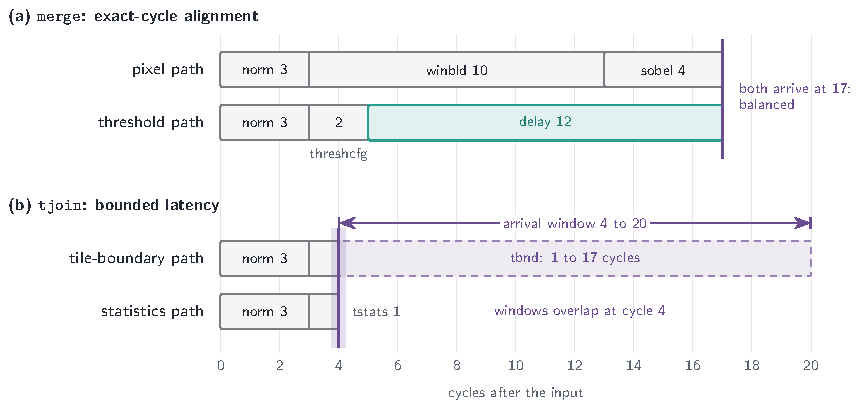
\includegraphics{figures/fig_forge_latency}
  \caption{Arrival times at two merges in the platform wrapper. (a) Both paths reach \texttt{merge} at cycle 17. The threshold path uses a fixed 12-cycle delay, which is also the delay \forge{} would select automatically. (b) The tile-boundary path reaches \texttt{tjoin} between cycles 4 and 20. That interval includes the statistics path's arrival at cycle 4.}
  \label{fig:forge:latency}
\end{figure}

A connection between clock domains must declare an adapter: a two-flop level synchronizer, a pulse synchronizer, a mailbox handshake, or an asynchronous FIFO, whose RTL \forge{} emits, or a waiver with a reason. An undeclared crossing stops generation. The latency graph adds two destination-clock cycles for a level synchronizer and three for a pulse synchronizer; mailbox and FIFO transfer times remain unknown. The checker uses declared latencies and keeps cycle counts from different clock domains separate. RTL latency, physical timing, and metastability require separate checks.

Static throughput analysis estimates the nominal capacity $rf/\mathrm{II}$ of a stage that accepts $r$ records per initiation interval at frequency $f$. A simulation probe samples FIFO status on one clock and reports occupancy and the average rate over the sampled interval. For multi-clock or enable-gated FIFOs, the project must count the transactions separately.

\subsubsection{Verification}
\label{sec:forge:verification}

For a \texttt{forge.yml} project, \texttt{forge test} reads the top name, clock, reset, RTL sources, and input and expected data. For link words, codecs can specify which bits encode each field. \forge{} reads the RTL ports, drives the inputs, and compares the specified output fields in each event, in order or as a set. The report gives the event, interface, cycle, and fields that differ. It records a missing packet against the event in which it was expected. Use \texttt{--event-id} to replay a single event. The testbench drives and reads HLS memory interfaces through the HLS memory protocol.

A plugin declares its verification flows for HLS C simulation, individual RTL modules, and the integrated payload. The RTL flows use a generated SystemVerilog testbench whose port bindings come from the current interface metadata. A flow may keep a hand-written port map, and \texttt{forge dev verify generate} compares its ports, directions, and widths with the RTL and stops if they disagree. The plugin interprets the dataset and supplies the reference-model provider and scoreboard. \forge{} invokes the provider, records hashes of the input and output, and runs the flow. RTL simulation uses AMD Xsim~\cite{AMD_Vivado_LogicSimulation_UG900} or Verilator. This infrastructure can host methodologies such as UVM~\cite{Accellera_UVM} but does not provide constrained-random stimulus or coverage closure. \texttt{forge report} collects topology, latency, throughput, and verification results into an offline HTML report without rerunning them.

\subsubsection{Board frameworks and existing projects}
\label{sec:forge:external-integration}
\label{sec:forge:core-isolation}

The \texttt{framework} commands load an external board framework's ABI and endpoint manifests and emit the payload wrapper around the generated top, matching links from manifest data. What a board needs beyond per-link wiring is declared as payload control policies rather than patched into the generated file: input and output registers, receive gates, configuration and status words mapped to framework registers, and the project's own Verilog blocks. A floorplan command assigns block-design cells to device regions from the resolved links. For an existing repository, \texttt{forge init} writes a minimal \texttt{forge.yml} and \texttt{forge adopt} scans sources and the instantiation graph, recording the decisions the scan cannot make; the adoption commands are covered by repository tests, and no third-party adoption is evaluated here. Commands that accept \texttt{--json} return a common envelope of status, diagnostics, artifacts, and metrics, with exit code 0 for a pass, 1 for a failure or a warning under \texttt{--strict}, and 2 for usage or internal errors.

\subsection{Operation}
\label{sec:methods:operation}

\subsubsection{System requirements}

\forge{} is an MIT-licensed Python package, version~3.0.0, with a \texttt{forge} command-line entry point. It requires Python~$\geq3.8$~\cite{Python_Language}, PyYAML~\cite{PyYAML}, and Jinja2~\cite{Jinja2}. Contract validation, structural generation, and static analysis do not invoke vendor tools. HLS synthesis and C simulation require Vitis HLS. The block-design output targets Vivado IP integrator. For RTL simulation, Xsim and Verilator are supported. Waveform and probe capture are available with Xsim. The main set of archived experiments used Linux, Python~3.9.25, PyYAML~6.0, Jinja2~3.1.6, Vitis HLS and Vivado~2024.1, and Verilator~5.022.

\subsubsection{A runnable example}
\label{sec:methods:implementation:workflow}

The \texttt{examples/cmssw\_reference} directory of the source contains a 100-event export of the CMS OMTF emulator, two codecs, and a small payload, \texttt{candidate\_to\_gmt.v}, that rewrites each link's track-finder candidates as Global Muon Trigger words. Its \texttt{forge.yml} is the complete description:

\begin{codeblock}
project: cmssw_reference
top: candidate_to_gmt
sources:
  rtl: [rtl/*.v]
clock: {port: clk}
reset: {port: rst, active: high}
verification:
  target: existing
  backends: [verilator, xsim]
  input: {path: data/input.txt, format: empv2, events: data/input.events.json}
  expected: {path: data/expected.txt, format: empv2, events: data/expected.events.json,
             provenance: data/provenance.json}
  links: {l0: 0, l1: 1, l2: 2, l3: 3, l4: 4, l5: 5, q0: 0, q1: 1, q2: 2, q3: 3, q4: 4, q5: 5}
  codecs:
    "q*": codecs/samuon.yml
  compare: {fields: [pt, eta, phi, charge, qual], order: event}
\end{codeblock}

With FORGE v3.0.0 installed, run these commands from the example directory to pack the export into pattern files, simulate the top, and write the report:

\begin{codeblock}
python3 make_patterns.py   # data/input.txt: 100 events, 217 candidates
forge test                 # Verilator and Xsim, whichever is installed
forge report               # .forge/reports/verification_results.md
\end{codeblock}

The Verilator result reports the number of matched and expected words on each link:

\begin{codeblock}[basicstyle=\ttfamily\scriptsize]
existing:candidate_to_gmt [verilator]: VERIFIED (q0 32/32, q1 35/35, q2 43/43, q3 38/38, q4 33/33, q5 36/36)
\end{codeblock}

To adapt the example, supply the new RTL and its reference export, and update the codecs and port mappings to match the design.
